\renewcommand{\prevpart}{0 }
\renewcommand{\thispart}{1 }
\renewcommand{\nextpart}{2 }

\section{Introduction to Machine Learning}

% Cover page
%
% Cover page for giveb part
%

\title[\modulename - Part \thispart]
{
  {\bf 
   \modulename - 
   Part \thispart\\
  }
  \vspace{0.5cm}
  {\it 
   \color{yellow}
    \secname\\
  }
}
\author[C.Andreopoulos] {
  Professor Costas Andreopoulos\inst{1,2}, {\it FHEA}
}
\institute[Liverpool/STFC-RAL] {
   \inst{1} University of Liverpool, Department of Physics\\
   \vspace{0.3cm}
   {\it {\color{magenta} Lectures delivered at the University of Liverpool, 2024-25}}\\
   \vspace{0.2cm}
}
\date{\today}

\titlegraphic{
  
\includegraphics[height=30px]{images/logo/liverpool.png}
}

\begin{frame}[plain]
  \titlepage
\end{frame}




% Outline
%
% Table of contents to be displayed at the beginning of each part
%

\begin{frame}[t,allowframebreaks]{Outline for Part \thispart -}
  % Part \thispart (\secname) covers the following topics:\\
  % \vspace{0.5cm}
  \linespread{1.1}
  \setcounter{secnumdepth}{3}
  \setcounter{tocdepth}{3}
  % \tableofcontents[currentsection, hideothersubsections, sectionstyle=hide/hide]
  \tableofcontents[part=\thispart]
\end{frame}



% Precursors
\subsection{Precursors of artificial intelligence}

% History of AI
\subsection{History of artificial intelligence}
\begin{frame}{The history of AI\footnote{
\tiny For a detailed discussion, see \url{https://en.wikipedia.org/wiki/History_of_artificial_intelligence}}}

\begin{itemize}
\item Birth of AI (1952-1956)
\item Symbolic AI (1956-1974)
\item First AI winter (1974-1980)
\item Boom (1980-1987)
\item Bust: Second AI winter (1987-1993)
\item AI (1993-2011)
\item Deep learning, big data and AI (2011-present)

\end{itemize}

\end{frame}



\subsubsection{Birth of AI (1952-1956)}

\begin{frame}[t,allowframebreaks]{Birth of AI (1952-1956) -} 

Several developments in the first half of the 20th century:
\begin{itemize}
    \item Discovery that the {\bf brain is an electrical network of neurons}
    \begin{itemize}
        \item 
          Richard Caton reported to British Medical Association 
          the first observation of electrical impulses from the 
          brains of living animals (1875) \cite{Caton:1875}.
        \item 
          Hans Berger recorded the first human 
          electroencephalogram (1924) \cite{Berger:1929}.
    \end{itemize}
    \item 
    Development of {\bf control and communication theory} (cyberneutics) 
    \begin{itemize}
        \item by Norbert Wiener
    \end{itemize}
    \item 
    Development of {\bf information theory} 
    \href{https://en.wikipedia.org/wiki/Information_theory}{\tiny [Wikipedia]}
    \begin{itemize}
        \item Early work by Harry Nyquist and Ralph Hartley in 1920's.
        \item Foundations established by Claude Shannon in the 1940's \cite{Shannon:1948}.
    \end{itemize}
    \item 
    Development of {\bf theory of computation} 
    \href{https://en.wikipedia.org/wiki/Theory_of_computation}{\tiny [Wikipedia]}
    \begin{itemize}
        \item John von Neumann, Alan Turing, Alonzo Church and others
    \end{itemize}
\end{itemize}

In early 1950's it became possible to start imagining a digital brain!

\framebreak

Landmark paper by \gls{Turing}\cite{Turing:1950tt} - Possibility of creating machines that think
Turing test

\framebreak

A first neural net machine, \gls{snarc}, 
was built by \gls{Minsky} and \gls{Edmonds} in 1951.

They drew inspiration from the work of 
\gls{McCulloch} and \gls{Pitts} on
artificial neurons.

\gls{snarc} was a randomly connected network of about 40 neurons (Hebb synapses)

Each neuron had a short-term memory and a long-term memory

The machine was trained by navigating a virtual maze (i.e. \gls{snarc} was a "mechanical rat").

Actions resulting to a positive reward (provided manually by an operator), 
engaged a chain that turned a potentiometer (whose setting was analogous to a weight in modern digital networks).

\begin{columns}
    \begin{column}{0.45\textwidth}
     \begin{center}
        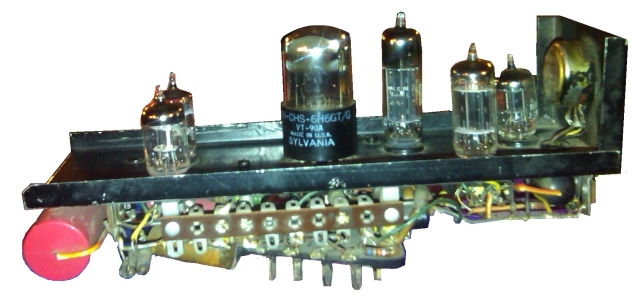
\includegraphics[width=0.99\textwidth]
        {./images/snarc/gregoryloan_snarc_hebbsynapse.png}\\
     {\scriptsize 
      A photograph by Gregory Loan of the only surviving \gls{snarc} neuron.\\
      \color{col:attribution} 
      Photo reproduced from \cite{CyberneticZoo:1951MazeSolver}}\\
     \end{center}
    \end{column}
    \begin{column}{0.55\textwidth}
    \end{column}
\end{columns}

\framebreak

Game AI and The Logic Theorist

\end{frame}




\subsubsection{Symbolic AI (1956-1974)}
\subsubsection{First AI winter (1974-1980)}
\subsubsection{Boom (1980-1987)}
\subsubsection{Bust: Second AI winter (1987-1993)}
\subsubsection{AI (1993-2011)}
\subsubsection{Deep learning, big data and AI (2011-present)}


%
%
%

\begin{frame}[t]{Effect of increased data}

    \begin{columns}
        \begin{column}{0.50\textwidth}
         \begin{center}
          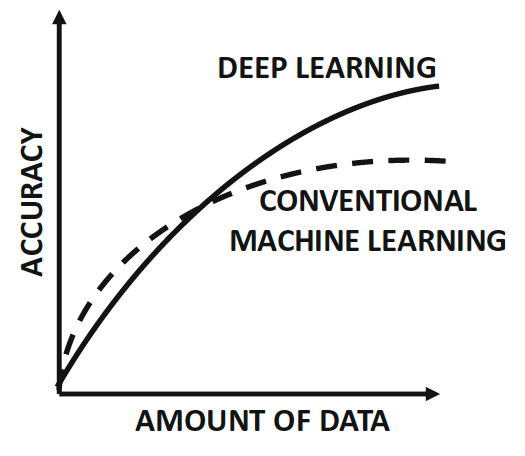
\includegraphics[width=0.95\textwidth]{./images/dl_intro/accuracy_vs_amount_of_data_1.png}\\
          {\scriptsize \color{col:attribution} 
          Image reproduced from p.54 of \cite{Aggarwal:2018SpringerDL}}\\
         \end{center}
        \end{column}
        \begin{column}{0.50\textwidth}
        \end{column}
    \end{columns}


\end{frame}

%
%
%

\begin{frame}[t,allowframebreaks]{Increasing neural network size - }

    % Intro

    % Number of connections in various artificial neural nets as a function of time
    % and comparison with biological brains

    The human brain has $\sim$100 billion neurons and $\sim$100 trillion synapses!

    \begin{center}
        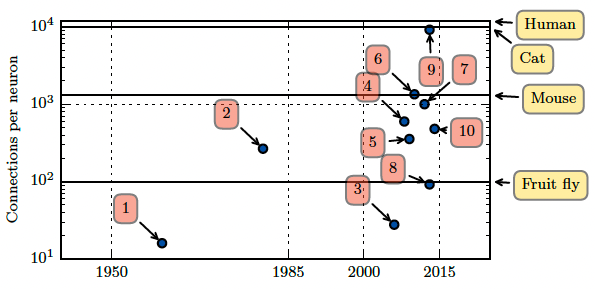
\includegraphics[width=0.95\textwidth]
          {./images/dl_intro/nnet_size_connections_vs_time_01.png}\\
        {\scriptsize \color{col:attribution} 
        Reproduced from p.22 of \cite{Goodfellow:2017DL}}\\
    \end{center}

    \framebreak

    % Number of neurons in various artificial neural nets as a function of time
    % and comparison with biological brains

    \begin{center}
        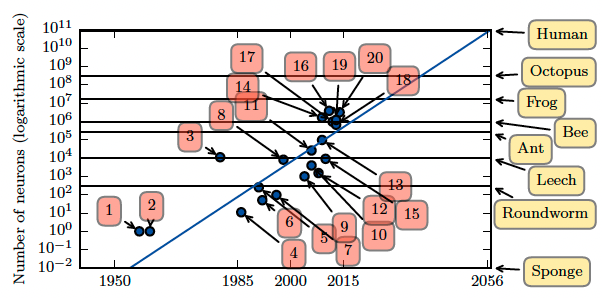
\includegraphics[width=0.95\textwidth]
           {./images/dl_intro/nnet_size_neurons_vs_time_01.png}\\
        {\scriptsize \color{col:attribution} 
        Reproduced from p.23 of \cite{Goodfellow:2017DL}}\\
    \end{center}
       {\tiny
       1. Perceptron (1958) \cite{Rosenblatt:1958p},
       2. Adaptive linear element (1960) \cite{Widrow:1960as},
       3. Neocognitron (1980) \cite{Fukushima:1980nc},
       4. Early back-propagation network (1986) \cite{Rumelhart:1986erp},
       5. Recurrent neural network for speech recognition (1991) \cite{Robinson:1991rerp},
       6. Multilayer perceptron for speech recognition (1991) \cite{Bengio:1991pma},
       7. Mean field sigmoid belief network (1996) \cite{Saul:1996mf},
       8. LeNet-5 (1998) \cite{LeCun:1998ln5},

       9. Echo state network (2004) (Jaeger and Haas, 2004)
       10. Deep belief network (2006) (Hinton et al., 2006)
       11. GPU-accelerated convolutional network (2006) (Chellapilla et al., 2006)
       12. Deep Boltzmann machine (2009) (Salakhutdinov and Hinton, 2009a)
       13. GPU-accelerated deep belief network (2009) (Raina et al., 2009)
       14. Unsupervised convolutional network (2009) (Jarrett et al., 2009)
       15. GPU-accelerated multilayer perceptron (2010) (Ciresan et al., 2010)
       16. OMP-1 network (2011) (Coates and Ng, 2011)
       
       17. Distributed autoencoder (2012) \cite{Le:2012daut}
       18. Multi-GPU convolutional network (2012) \cite{Krizhevsky:2012img},
       19. COTS HPC unsupervised convolutional network (2013) \cite{Coates:2013cots},       
       20. GoogLeNet (2014) \cite{Szegedy:2014gnet}\\
       }

    \framebreak

    % Information from recent well-known artificial neural networks

    \begin{itemize}
        \item GPT-2 had 1.5 billion parameters and around 50 billion neurons
        \item GPT-3 is estimated to have around 60-80 billion neurons
        \item GPT-4 is estimated to have around 60-80 billion neurons
    \end{itemize}

\end{frame}


\subsection{Human vs computer learning}

\subsection{Different learning paradigms: Supervised, unsupervised and reinforcement learning}

\subsection{Artificial intelligence, machine learning and deep learning}

\subsection{Machine learning tasks}

\subsection{A simple practical example: Linear regression}

\subsection{Biologically inspired methods of computer learning}

\subsection{Basic architecture of neural networks}

\subsection{Fundamental concepts}
\begin{frame}[t,allowframebreaks]{Fundamental concepts - }

    \gls{relu}
\end{frame}


% From AI to DL
\begin{frame}{Connection between AI, ML and DL}

\index{AI}\index{artificial intelligence}\gls{ai} -
\gls{ai}
\gls{ml}
\gls{dl}

    \begin{center}
        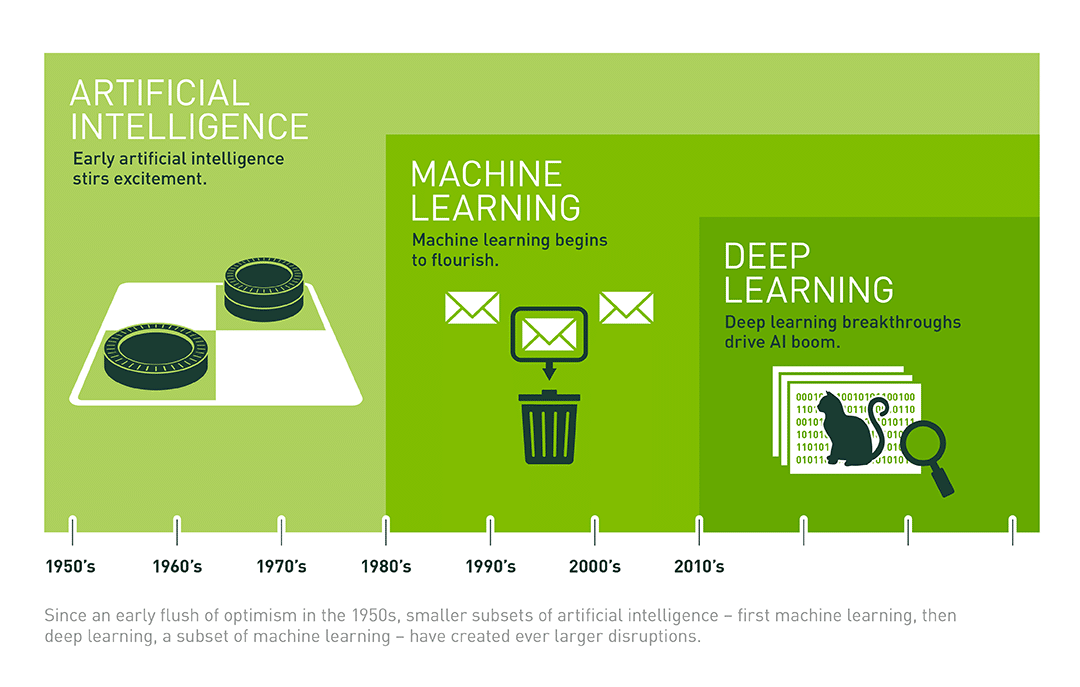
\includegraphics[width=0.90\textwidth]{./images/dl_intro/ai_ml_dl.png}\\
        {\scriptsize Image reproduced from \cite{NVidiaBlog:DifferenceBetweenAIMLDL}}\\
    \end{center}

\end{frame}
    


% Main points to remember
\renewcommand{\partsummarytitle}{Main points to remember }
\renewcommand{\summarizedlecture}{1 }

%
%
%

\begin{frame}{Lecture \summarizedlecture - \lecturesummarytitle}


\end{frame}



% Preview of next part
\begin{frame}{Preview of Lecture \nextlecture}

\begin{itemize}
{\small
\item blah
\item blah
}
\end{itemize}

\end{frame}



% References and suggested reading for this part
%
%
%

\begin{frame}{Suggested reading for Part \thispart}

    {
        \small
        Essential reading on {\bf automatic differentiation}:
        \begin{itemize}
            \scriptsize
            \item Section 6.5 from the `Deep Learning' 
            textbook of Goodfellow, Bengio and Courville \cite{Goodfellow:2017MITDL}.
            \item Appendix B from the `Machine Learning Refined' 
            textbook of Watt, Borhani and Katsaggelos \cite{Watt:2016Cambridge}.
            \item `A review of automatic differentiation and its 
            efficient implementation' by Margossian \cite{Margossian:2019ad}
        \end{itemize}
        
        Also, you may want to browse:
        \begin{itemize}
            \scriptsize
            \item The collection of articles
             in the book `Automatic Differentiation: Applications, Theory, and Implementations'
             edited by B{\"u}cker, Corliss, Hovland, Naumann and Norris \cite{Bucker:2005ABo}
        \end{itemize}
    }
    

\end{frame}

% Optional material


